\documentclass[]{report}
\usepackage{listings,graphicx}
\usepackage{float}
\graphicspath{{resources/}}

% Title Page
\title{WhisPeerer \\A WebRTC communications application}
\author{Dominic Rathbone \\ Student Number: 12843140 \\ Source Code: \\ https://github.com/domr115/CI360-Mobile-App-Dev}


\begin{document}
\maketitle

\tableofcontents

	\chapter{Introduction}
	The aim of this project was to provide an application enabling users to communicate using peer-to-peer technology. The motivation behind this was the increasing concern of security many consumers face in the modern age due to third parties, whether it be a corporation such as Facebook or an authority such as the UK Government, having access to and analysing their data. By using a technology called WebRTC, it is possible for two users to form a direct peer to peer connection over the internet.  Although a server is used for the initial signalling and negotiation process between the peers, the data sent over this peer to peer connection formed by WebRTC is never disclosed to an external server. On top of this, the application aimed to provide a sense of anonymity and impermanence by only providing users with a temporary, random unique identifier for a user-name and only storing data within the lifespan of it's application.

	\chapter{Development}
		\section{Node.js Signalling Server}
			\subsection{API}
			In order to set up a space in which two users can exchange the meta-data needed for the negotiation of a WebRTC peer connection, an API was created on the server using Express.js, a popular web application framework for Node.js. This consists of two endpoints, one endpoint to create a new user and one endpoint to check if the user exists. The former returns a unique, random session identifier to the application and the latter simply returns a status code of 200 or 404 dependent on whether the user exists or not. This API was designed using the Representation State Transfer (REST) architectural style in order to provide a uniform and consistent API to it's consumers. REST achieves this by modelling the endpoints in an API around the resources they represent with HTTP verbs representing the operations that are achievable on the resource. For example, in order to create a user on the server, the consumer send a POST request to a "/user" endpoint and in order to check if a user exists, the consumer sends a GET request to "/users/[userId]". This architectural style also makes the API more extensible as it is easy to design and add new endpoints to it.
			
			\subsection{WebSockets}
			To provide a bi-directional communications channels for the two application instances to negotiate the peer connection over, a WebSockets implementation called Socket.io was used. Socket.io models communication using the concepts of name spaces and rooms where a name space is represented by the endpoint a socket connects to and rooms are channels within this to which users can join and leave. In this case, each user is represented by their own name space "/user/[userId]". When another user wants to communicate with a user, they join this user's name space, becoming a "guest". In turn, this puts it into a "busy" state preventing other users from joining. From this namespace, the two users can exchange messages and once they are done and the guest disconnects, it is taken out of the "busy" state. By modelling the user's communications channels like this, the guest user can still receive incoming chat offers from a user whilst busy with another user, similar to how a mobile phone can still receive calls whilst in a call with another. 
			
		\section{Android Application}
			
			\subsection{Architecture}
			As the majority of the data processing is handled by the libraries the application is dependent upon, it's responsibilities mainly lie in the triggering of and reaction to incoming messages from another instance of the application, whether it be through the signalling server or directly via the peer-to-peer connection. Due to this, the architecture of the application can be represented by an "Event-Driven Architecture" pattern. This is where the flow of control in an application is dictated by the emission of and reaction to "events" where an event is a change in the state of the application. The overall architecture of the system the application is a part of can be broken down into 3 layers, the presentation layer, the communications layer and the server with the communications layer being the basis on which the user interface retrieves information from another instance of the application.
			
			\begin{figure}[H]
			\caption{Application Architecture}
			\includegraphics[scale=0.2]{Architecture.png}
			\end{figure}	
					
			\subsection{Design Patterns}
			To create the event-driven architecture, the application utilises the Observer pattern to trigger changes in the flow of the application by asynchronously updating activities (and thus the user interface) when certain events are received. The observer pattern is a design pattern in which two types of objects are implemented, "Observers" and "Observables". Each Observer overrides a set of methods that are called when an event on the "Observable" object happens and then adds itself to a list of observers on that observable object. When an event occurs on this observable object, it goes through the list of observers, calling their corresponding implementation of the method (see appendix A, section 1 for an example). In this case, the observer pattern was chosen as activities such as the one that represents an incoming call activity needed to be instantiated spontaneously throughout the application. By using the observer pattern, the current activity could assign itself as the observer for the signaller (implementing the observable interface), updating it when the signaller received an "offer" for an incoming call. 
			
			As the majority of the "events" within the application took the form of JSON messages transmitted and received from another application instance over the WebSockets connection, the Java client library for Socket.io also used the Observer pattern. However, as the library was the one supplying the observable objects. The application only needed to supply the observers by passing through anonymous classes implementing the library-specific "Listener" interface when setting up these events. This interface requires the object to implement methods with the code that is to be called when the event is received (see appendix A, section 2 for an example). Further to this, the application also interacts with the server through a HTTP API, prior to establishing a signalling session with WebSockets. To react to a success or failure of the requests sent to the API, a handler is passed through implementing methods with the code that should be executed in these cases (see appendix A, section 3 for an example).
			
			The application also uses the factory pattern in order to produce media streams to send to the other user through the peer connection. The factory pattern obfuscates the process of creating these media streams away from the object that called them, meaning it only has to supply the options for the object they want the factory to create (in this case, a parameter is passed through specifying whether a video stream should be added).
			
		\section{Communications Layer}
		To communicate with the server and other application instances, the application makes use of various libraries to implement a number of communications protocols. 
		
			\subsection{Android Asynchronous HTTP Client}
			The first of these is the Android Asynchronous HTTP Client library. This library was used as it made it easy to send asynchronous HTTP requests to the node.js server. A static class was created that mapped each endpoint of the HTTP API to a method which the activities could then call, passing parameters such as a username and a handler with the code that they wanted executed when the result was returned. The library then executed this request by adding it to a queue from which a pool of threads picks from, passing through the handler with it.
	
			\subsection{WebRTC/LibJingle}
			The application uses WebRTC to form a peer-to-peer connection using a offer-answer negotiation process. The offer and answer are formatted using the "Session Description Protocol" (SDP) and contain the parameters that represent what each peer wants from the connection such as media constraints (See Appendix B for an example). The initiating application creates a peer connection object and then an "offer" SDP which is sent over WebSockets to the server which forwards it on to the destination application. This application, listening for socket events, receives the SDP and sets it as the remote description. After doing so, it generates an "answer" SDP and sends it back to the offerer through the same channel. Once they both have the SDPs, the library can extract the parameters from them to connect the two peer connection objects. From this, the application creates a media stream that can contain the live streaming video from the camera and the audio from the microphone and adds it to this peer connection. This media stream is sent over a protocol called SRTP. SRTP is an extension to the real-time protocol (RTP) that provides more security features such as authentication and encryption. RTP is a protocol that usually sits on top of the UDP transport protocol and is used for media streaming over a network and therefore is primarily used in telephony and video conferencing applications. Although it uses UDP and thus doesn't provide any mechanisms for reliability or quality of the data in the stream, it is supported by another protocol called Real-Time Control Protocol (RTCP) which monitors the transmission of data in order to provide statistics on the quality of service provided by RTP. This way, the statistics can be sent to participants of the stream and measures can be taken to detect and fix faults in this transmission. 
						
			
			\subsection{Socket.io Java Client}
			To provide a method of bi-directional communication that is necessary for the negotiation process used by WebRTC, the server uses Socket.io. To support this on the client application, it uses a un-official library that is based on the official Socket.io java engine library to provide an interface into it. In turn, this library uses HTTP to upgrade the connection between the Socket.io server and the client to use the WebSockets (WSS) protocol, from which it can send messages to or receive messages from the server. If this upgrade is not possible, it falls back on long polling the server using HTTP requests. WebSockets was chosen as the protocol for bi-directional communication as even though the application is not browser-based at the moment, if the platform was expanded to include a browser-based web application, it would mean that the android application would be able to communicate with it. If the communication was implemented with plain TCP sockets instead, this would not be possible.
		
		\section{Presentation Layer}
		Using the observer pattern described earlier, each activity making up the presentation layer is able to subscribe to parts of the communication layer for updates from the server and other application instancse whilst also sending updates through it itself. 
		
		\begin{figure}[H]
			\caption{Application Flow}
			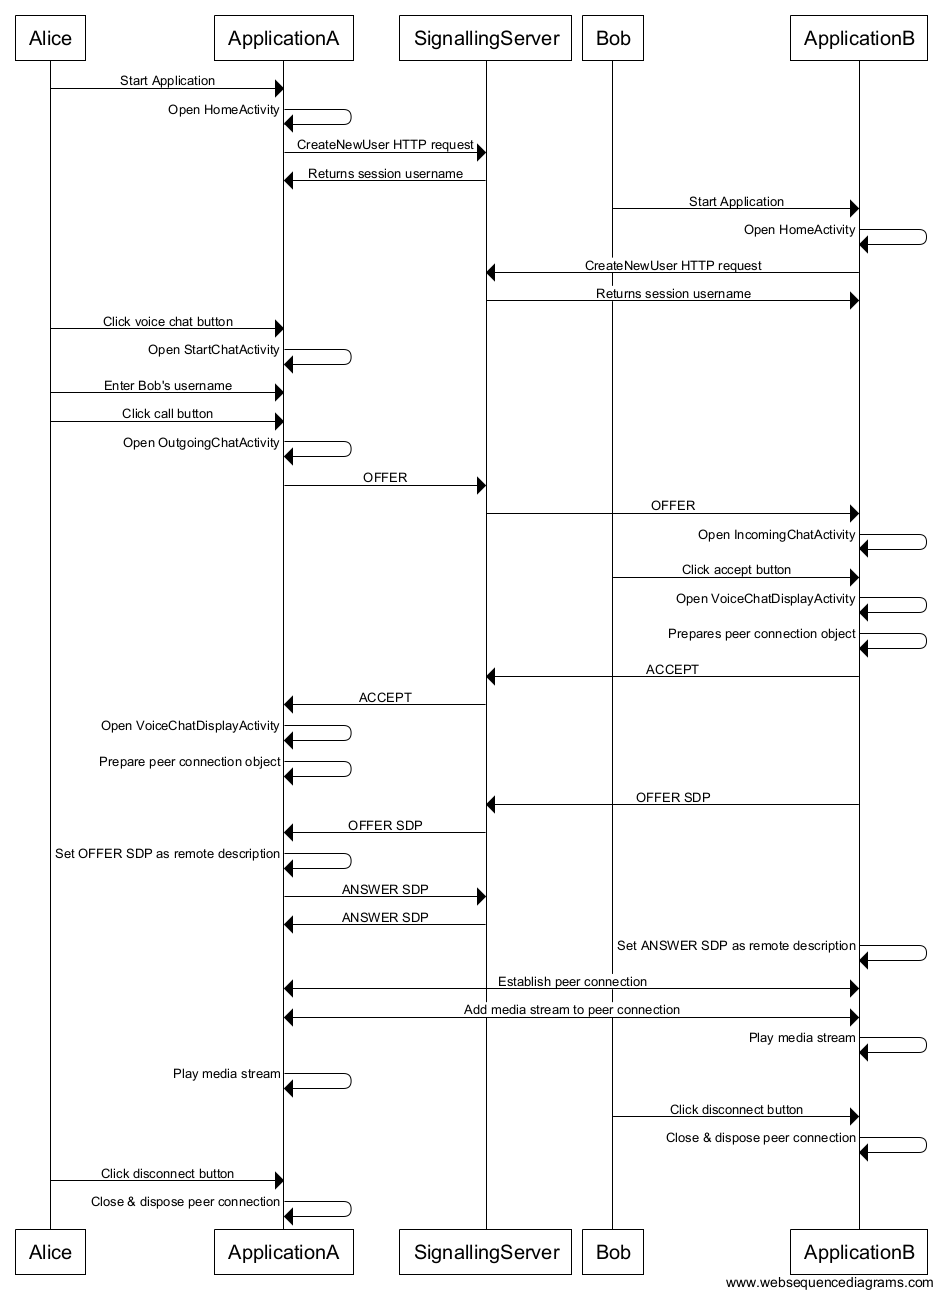
\includegraphics[scale=0.3]{ApplicationFlow.png}
		\end{figure}	
					
		\subsection{Home Activity}
			\begin{figure}[H]
				\caption{Home Activity}
				\centering
				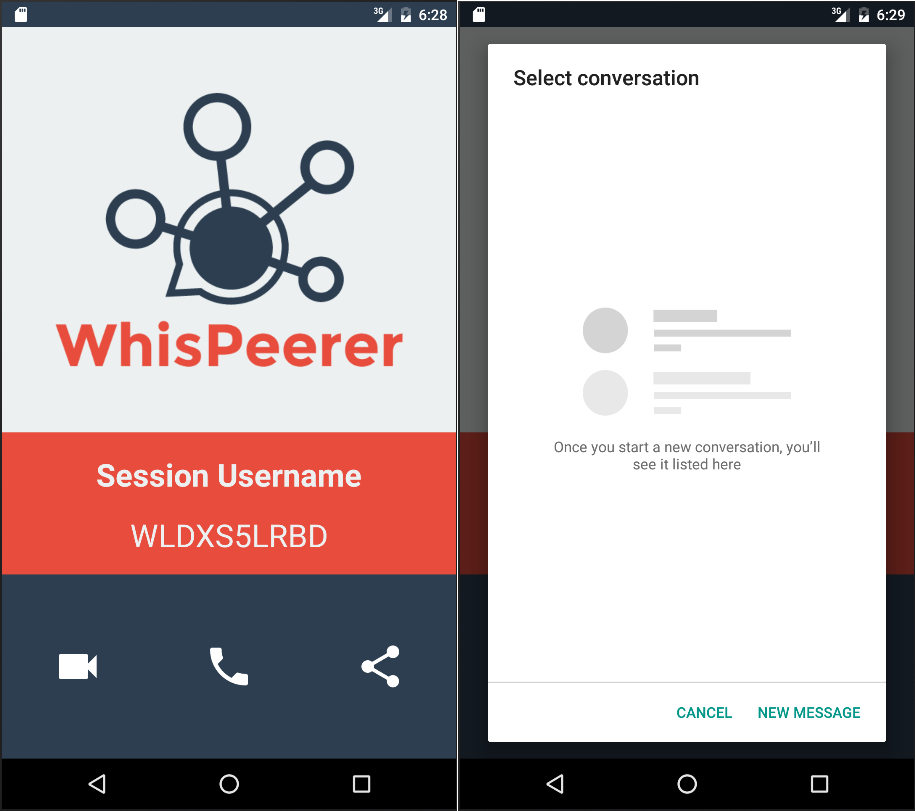
\includegraphics[scale=0.35]{HomeActivity.png}
			\end{figure}		
		The home activity is the entry point into the application. Due to this, this is where the application is se tup to be able to receive messages from another instance. To do this, a HTTP request is sent to the server, creating a name space in which other users can connect to with WebSockets. The response to this request returns a unique identifier for the user's session. With this unique identifier, the application connects to the name space by creating a new Signaller instance, setting itself as the observer to this instance so it can listen for incoming events. From this activity, the user can either initiate the process to start a video or voice chat as well as share their session username via the pre-defined android share intent. Clicking the share button will open a pop-up in which the user can select an application to share their session user name through.
		
		\subsection{Start Chat Activity}
		\begin{figure}[H]
			\caption{Start Chat Activity}
			\centering
			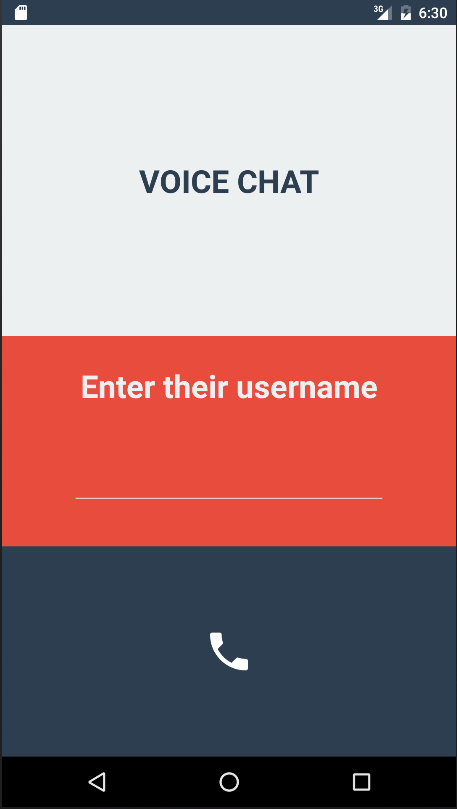
\includegraphics[scale=0.35]{StartChatActivity.png}
		\end{figure}
		When the user decides they want to either video or voice chat with someone, they open the Start Chat Activity by clicking the corresponding button on the home activity. Both of these buttons open the same activity but pass through a different "Chat Type" string extra with the intent, distinguishing their routes through the application. On this screen, the user can enter the session username of another user currently in the application in order to start a chat with them. Hitting the call button will send a HTTP request to the server, checking if the name space that defines the user exists. If it doesn't exist, it will trigger an error on the interface but if it does, it triggers the opening of an "Outgoing Chat" activity.
		
		\subsection{Chat Activity}
			\begin{figure}[H]
				\caption{Chat Activity}
				\centering
				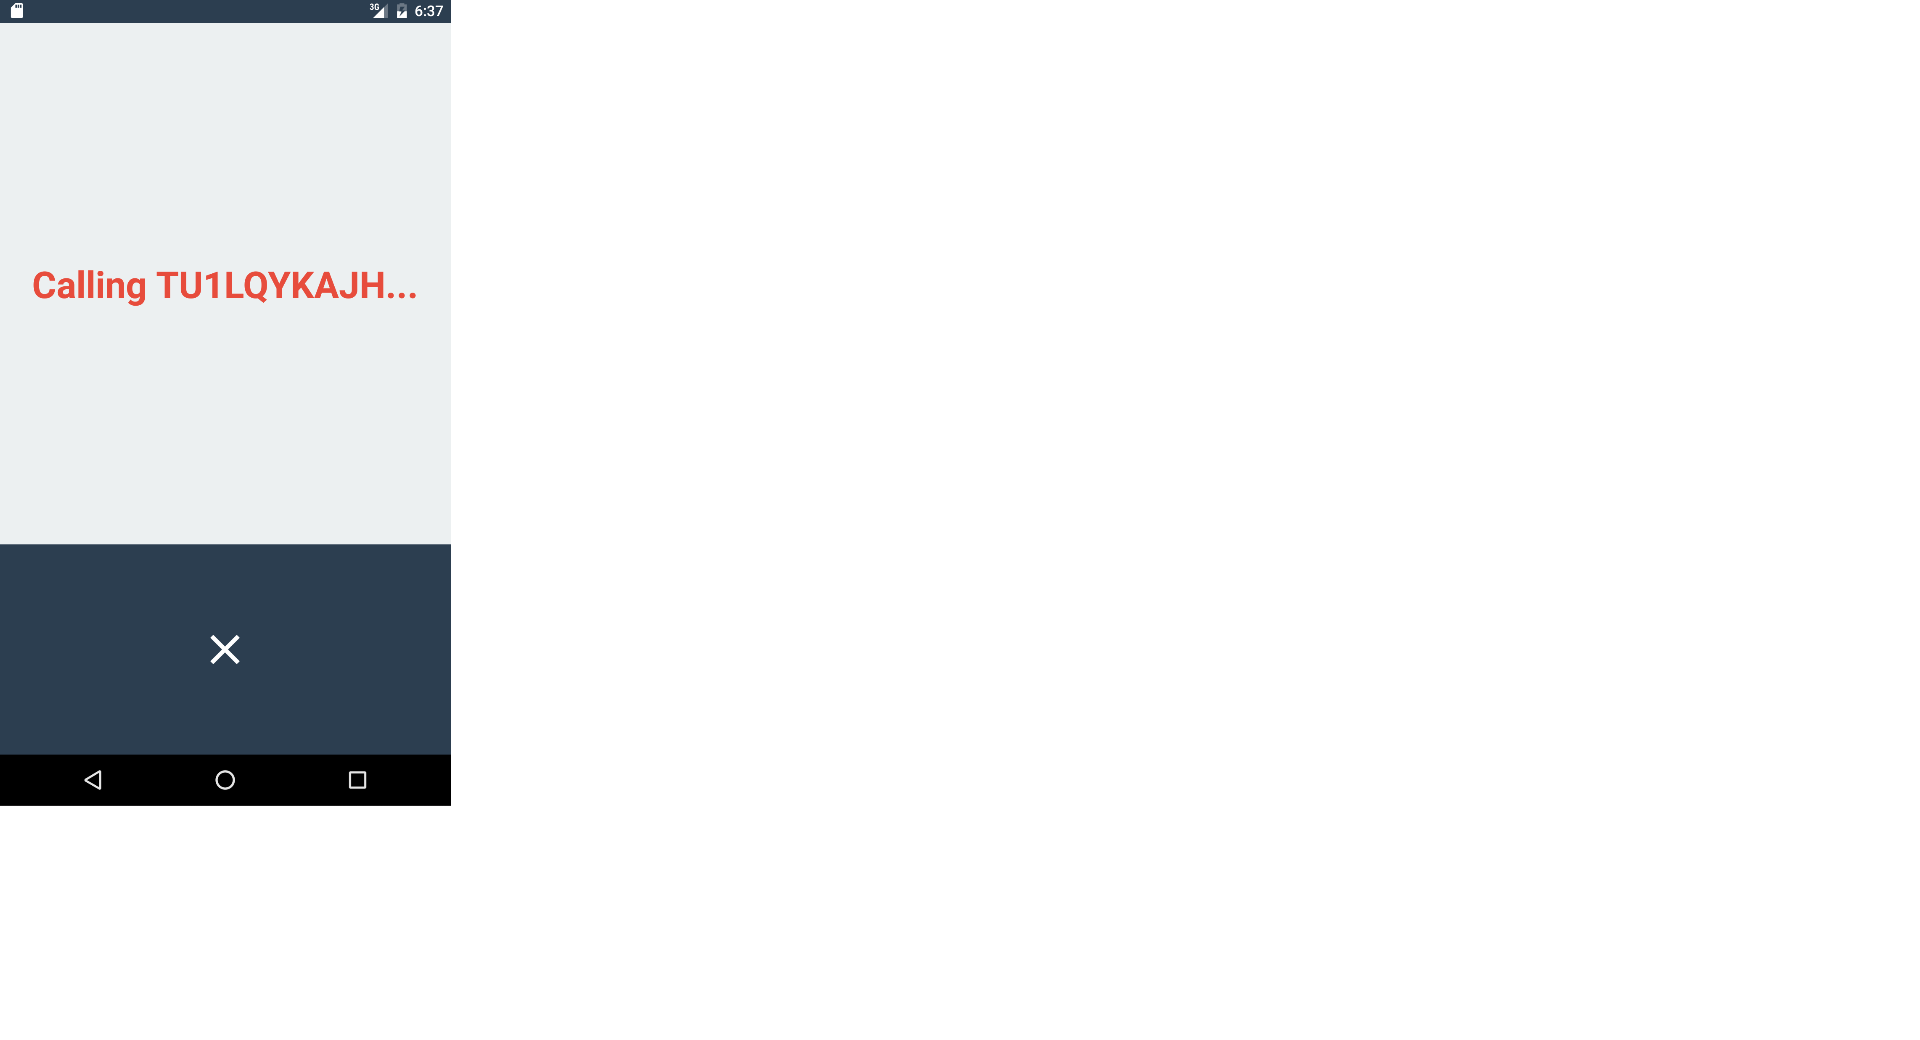
\includegraphics[scale=0.35]{ChatActivity.png}
			\end{figure}
		The chat activity is sub classed by two classes. The first subclass activity represents an outgoing chat request to another user. When the user enters this activity, it sends an initial "offer" message to the destined application via WebSockets, initiating the chat process. However, the user can also cancel this offer by clicking the cancel button which sends a "cancel" message to the destined user, telling them to stop this process on their side as well as finishing the activity. If the destined application doesn't respond within 17.5 seconds, it automatically sends this "cancel" message as well.
		
		When the destined application receives the initial offer message, if they are in an activity currently subscribed to the signaller and is listening for the "offer" event, it will trigger an instance of the Incoming Chat activity (the second subclass of the chat activity) to be created. From this, the user can either click accept or decline. Clicking the decline button sends a "declined" message to the offerer but clicking the accept button triggers the application to open a chat display activity.
		
		\subsection{Chat Display Activity}
			\begin{figure}[H]
				\caption{Chat Activity}
				\centering
				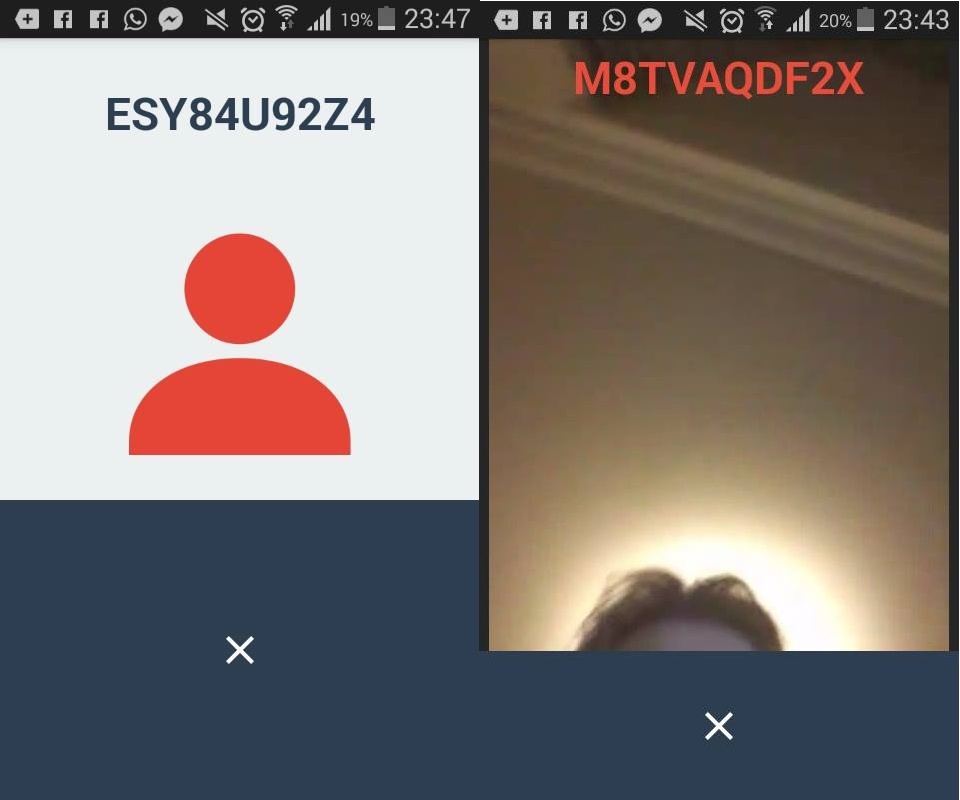
\includegraphics[scale=0.35]{ChatDisplayActivity.png}
			\end{figure}
		
		The chat display activity class is also sub-classed by two others, one subclass for a video chat and one for a voice chat, the main difference between them being how they prepare for and play the incoming media streams. From the chat display activity, each user sets up their peer connection object and creates the media streams that they are going to send to the other. Once the answerer application has done this, it sends an "accepted" message to offerer and listens for the offer SDP to be sent, triggering the offer-answer negotiation process. Once a peer-to-peer connection has been achieved, each user listens for the media stream to be added. In the video chat display activity, in order to render the video stream on the screen, it uses an OpenGL component called a "GLSurfaceView", this is an implementation of a regular SurfaceView but allows for rendering with OpenGL instead of plain 2d rendering. Once the stream has been received, it is added to the GLSurfaceView, rendering it for the user. The voice chat display activity is much simplier as doesn't need to render anything on screen and simply has to enable the audio stream when it is received. To produce these media streams, the chat display activity calls the MediaStreamFactory class, supplying it with the parameters based on whether it is a video chat or a voice chat. This factory returns a wrapper object containing the media stream as well as the video source and the audio source so that when the user disconnects, these can be disposed of.
		
		\section{Android Hardware}
		In order to produce the media streams, the application had to access both the camera and the microphone of the device. To do this, the application has to ask for access to these when the application is installed. However, in the newer versions of the android SDK, the application also has to ask for permission on the activity that uses them. As a result, the chat display activity has to ask for permissions before it can create media streams from the microphone and camera output. Another service the application uses is the android vibrator used in the incoming chat activity to alert the user that they are receiving a chat.
		
		\section{Manual Testing}
		As the majority of the application focused on asynchronous interactions between the presentation and communications layers, it was hard to implement a suite of automated tests as the majority of these automated tests would require mocking a lot of the dependencies that most of the methods relied on. On top of this, unit tests seemed relatively pointless as most of the methods in the application didn't process any data, so there was not a lot of output to test and on top of this, they would have taken a lot of time to produce. 
		
		Instead, as the application is relatively complicated in how it performs certain tasks, a manual testing process was used in which the application was black-box and white-box tested. The former being when the application is tested without any knowledge of it's internals and the latter being where the internals are known. In this case, the black box tests consisted of running the applications without debugging them to see if there were any small usability faults with the them. The white box tests were used as the main method of testing and these consisted of debugging the code as the application was being used to ensure that it was working correctly. The application was tested on a Samsung tablet running Android Jelly Bean and a Samsung smart phone running Android KitKat as well as emulators running Lollipop and Marshmallow. Testing on various versions meant that more faults were able to be found before release but by increasing the amount of supported versions, this also means that more development time had to be put in and there is a bigger chance for undetected bugs to occur.
		
	\chapter{Design}
		As the application used relative new and experimental technologies, the majority of the project was focused on developing these to ensure they worked. On top of this, the routes through the application are relatively simple meaning less effort was needed to ensure the user knew them. Due to this, the design aspect of the project was considered a lower priority. However, taking account for this, time was still spent in order to produce a modern and clean look. To make this easier, aspects of Google's material design guidelines were taken advantage of including their default icon set.
		
		\section{Layout}
		The application mainly uses relative and linear layouts for structure. This structure was inspired by how traditional call applications work in order to make the user feel familiar as soon as they start it. By doing so, it meant that there did not have to be as much information on the screen to show the user how the application worked. The layout of the application is based around blocks arranged vertically on the screen, distinguished by their color. These blocks separate the information and interactive components within the activity to provide a simpler user experience. 
		
		\begin{figure}[H]
			\caption{Block Layout}
			\centering
			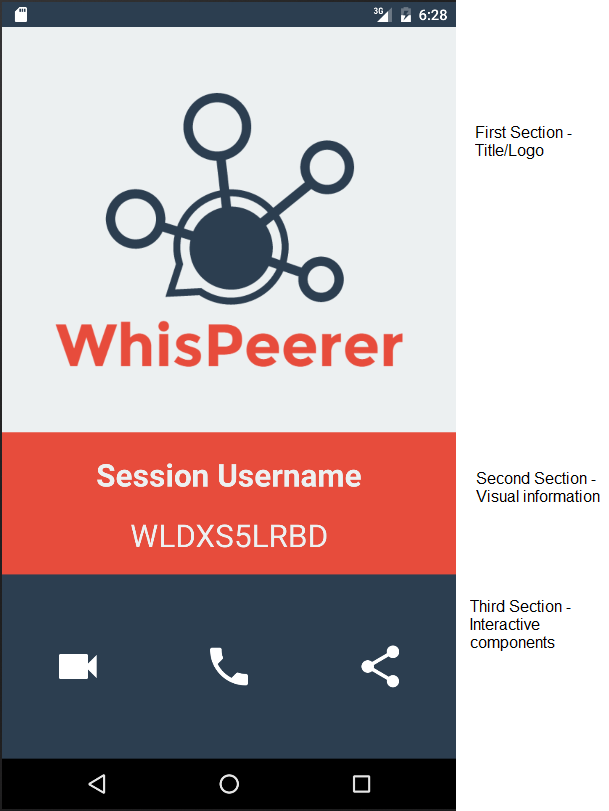
\includegraphics[scale=0.35]{blocks.png}
		\end{figure}
		
		The first section is to provide context to the activity. For example, in the Home Activity, the first block tells the user the application they have just entered. The second block then tells them the information they need for the application. The most important block is the third, in order to replicate the design of a traditional call application, the main functionality of every activity is arranged in a tool-bar style block at the bottom of the screen. This allows for the user to easily reach for every button with just one hand holding the device, making it more convenient especially when you are in a call. The third block is consistent across all of the activities but not all of them contain the second block as that level of interaction is not always needed such as in the Voice Chat Display Activity.

		\section{Colour Scheme}
		\begin{figure}[H]
			\caption{Colour Scheme}
			\centering
			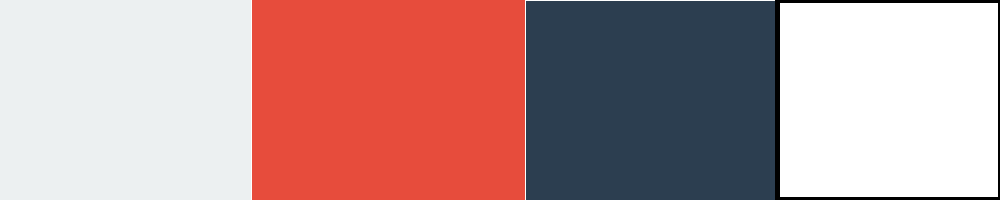
\includegraphics[scale=0.35]{ColourScheme.png}
		\end{figure}
		The colours in the scheme were chosen as they complement each other whilst also being distinguishable so they can be used to form blocks in each activity. The grey colour is used as the primary background color throughout the application, the red colour indicates an element of important information or interactivity that the user should pay attention to and the blue colour is always used to signify the tool bar. This was done to give the user a consistent experience throughout the application with the hope that they begin to associate the colours with certain actions or prompts.
		
		\section{Logo}
		\begin{figure}[H]
			\caption{Logo}
			\centering
			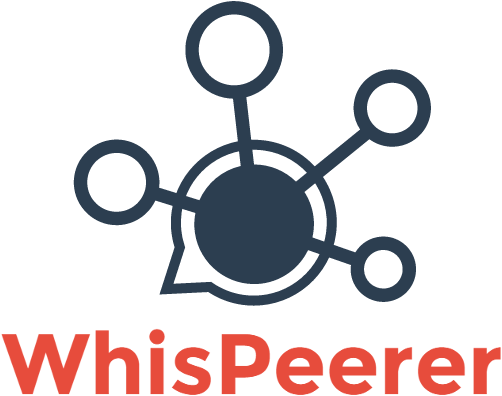
\includegraphics[scale=0.35]{logo.png}
		\end{figure}
		The logo was created to represent the functionality of the application, albeit in a relatively abstract way. It is a combination of a "speech bubble", a well known symbol representing that the application is used to talk to people as well as a topology diagram of a set of nodes in a network representing that the main focus of the application is supplying this chat functionality via a peer-to-peer connection.
		
		\section{Icons}
		\begin{figure}[H]
			\caption{Icon Set}
			\centering
			
\includegraphics[scale=0.35]{iconset.png}
		\end{figure}
		The icons used in the application are mainly taken from Google's material design icon set and were chosen as they are already ubiquitous through application design, again adding to a sense of familiarity as a user can go into the application knowing which icons are associated with certain calls to action. For example, the phone symbol is universally known as the call to action for a phone call. 

	\chapter{Reflection \& Review}
		\section{Background Research}
		The background research that was undertaken before the project was began definitely gave me context of how WebRTC can be used to build a mobile application to an extent. However, as the technology was built for the browser and ported to the android platform unofficially, there was a lack of documentation that I could have referred to throughout the process to help me understand it's intricacies, instead having to rely mainly on pre-built demo applicationsas a reference point. This resulted in having to spend a significant amount of time working on faults that had major effects on the application but actually had relatively simple solutions.
		
		An example of this is the calling order of asynchronous callbacks when creating, setting and receiving SDPs. The lack of documentation meant that I spent almost a week and a half figuring out why the application was sending two copies of their SDP as opposed to one when the problem was that the callback triggered on the successful setting of an SDP was called when both the local and remote SDP were being set. This meant that the offerer would create and set an offer as their local SDP, send it out, receive an answer, triggering the callback again, sending out another offer and then receiving another answer in reply. This resulted in two instances of an application activity being opened and often caused the application to crash. The solution was relatively simple as all I had to do was add statements to distinguish between incoming and outgoing SDPs in the callback but as it was asynchronous, it meant that it was extremely hard to debug and detect without documentation.
		
		Further to this, I did not do enough background research into the technologies that played a smaller role in the application. For example, I did not look into the OpenGL GLSurfaceView component, which meant that when it came time to render the video stream on an activity, a lot of time was spent making this work. One of the problems I had with this was that the video stream was coming from a front-facing camera meaning that it natively renders at a 270 degree angle. In order to display this on screen, I had to change the dimensions of it in order for the user to be able to use it in portrait mode.
		
		\section{Methodology}
		At the start of the project, I followed the methodology plan relatively well by using the Kanban board to analyse my progress. However as time went on, I stopped following this so much due to the application becoming more complex, resulting in the majority of my time experimenting with the technology in order to fix the problems I had faced. I felt that this was a reasonable sacrifice to make in order to focus on the actual development of the application as I would have most likely spent just as much time organising the development process as I did on the application itself due to how many changes I was making a day. However in hindsight, these problems would probably have occurred less often if I had stuck to the methodology and workflow board more rigorously.
		
		\section{Testing}
		Had there been more time, I would have created a suite of automated integration tests in order to ensure that each component worked together. On top of this, I would have also added unit tests to the Node.js signalling server using the Mocha framework and would have also created a suite of tests for the API with a tool such as Postman or Advanced Rest Client. These changes would have saved me time in detecting and fixing bugs as I would have been able to run them whenever a change was made, ensuring that no functionality was broken which would have also make the application easier to extend in the long run.
				
		\section{External Technologies}
			\subsection{Git}
			Throughout the development process, I made back-ups of the changes I made by committing them to a GitHub repository via the git CLI. This allowed me to track my work and log the changes throughout the lifespan of the project as well as revert changes if I had made a mistake. By getting into the habit of doing this, I was able to work on my project on different machines without having to carry around some sort of portable storage device with me. Although, I could have used a cloud storage service such as dropbox, this does not offer the same revision control that git does. Having my work in a git repository also allows me to easily share my work with my assessors as well as other interested parties such as employees or potential contributors.
			 
			\subsection{Development Environments}
			Android Studio made the development of my application extremely easy as it aggregated all the tools I needed to use into one development environment instead of, for example, having to run the android emulator manager on it own. This convenience meant I spent less time setting up tools and more time on developing the application. To develop the Node.js I used WebStorm, an IDE created by JetBrains, the same company that makes the Java IDE that Android Studio is based on. This was very similar to Android Studio which meant that I spent less time acclimatising between the two development contexts and languages.
			
		\section{Application Improvements}
			\subsection{Web to Native Application Communication}
			One extension of my project that would truly make it unique would be creating a web application for it. The major advantage of using WebRTC as a communication protocol as opposed to other VoIP solutions is that is can be used to connect users in browser-based applications with users in mobile applications. By creating a JavaScript application that uses the same signalling server, users could communicate cross-platform through a peer-to-peer connection. On top of this, if an iOS and desktop application were made for the platform, it could provide a truly ubiquitous service that would not limit anyone from using it.
			
			\subsection{Media Quality}
			A major improvement of the application would be optimising the video and audio streams to maximise quality. At the moment, the audio quality is relatively mediocre particularly as it suffers from the larsens effect (where an audio output such as a speaker can hear the audio input, creating a feedback loop). Although the audio stream does have the default android echo cancellation pre-processor ran on it it, it hasn't seemed to fix this problem.  A simple way of improving this in voice chats would be to make the media stream quieter so the user has to put the phone to their ear to talk. However, this wouldn't solve the problem in video chats where the users need to be able to see each other so other more complex solutions would have to be introduced such as a custom-built cancellation pre-processor for the application. The quality of video streams is also hard to improve as they have a hard limit by the maximum frame rate and resolution of the camera involved. They also have a soft limit that could be exceeded but at the expense of performance by, for example, modifying the bit rate of the stream.
			
			\subsection{Camera Switching}
			At the moment, the users are limited to only use their front-facing camera to capture video. The user experience could be improved by presenting the user with an option on the Video Chat Display Activity that would let them switch between the front and back-facing cameras during the chat. This option is currently supported by the WebRTC API so it could be implemented relatively easily.
			
			\subsection{Local Media Stream Rendering}
			The application is also lacking a feature seen on many modern video call applications which is the ability to see a user's own stream. The application should not only display the remote user's stream but also their own stream in a smaller GLSurfaceView component. This would improve the user experience of the application greatly as it provides the user with feedback on how well their stream is playing.
			
			\subsection{Media Controls}
			The final limitation of my application is that it doesn't have any form of controlling the streams such as a mute or pause button. Adding these would make it more complete user experience and would make it a better competitor to current solutions 
						
			\section{Conclusion}
			The main conclusion I came to during the process of creating this application is the realisation that WebRTC is still very much in it's early stages. This means that although the application is a great prototype to demonstrate the technology's abilities, it does not yet provide a valid alternative to well established technologies such as Skype's VoIP implementation or even the browser implementation of WebRTC. The lack of an official Android WebRTC API is the main limiting factor in this as it means there is not an industry standard from which WebRTC Android applications can be built, particularly due to the lack of documentation in the unofficial ports.
			Saying this, the opportunity to use WebRTC to produce a mobile application was enjoyable and definitely presented a novel and extremely challenging development experience for me from which I learnt a lot.
				
	\appendix
	\chapter{}
	\begin{figure}[h!]
		\caption{Observer Pattern}
		\begin{lstlisting}[language=Java,frame=single,breaklines=true]
		
public class HomeActivity extends AppCompatActivity implements Observer {
	@Override
	public void update(Observable observable, Object data) {
		log.v("observer", (String) data);
	}
}

public class Signaller extends Observable {
	Observer observer = null;

	public void setObserver(final Observer observer) {
		this.observer = observer;
	}

	public updateObserver() {
		observer.update(this, "UPDATE TIME");
	}
}
		
		\end{lstlisting}
	\end{figure}
	\begin{figure}[h!]
		\caption{Socket Event Listener}
		\begin{lstlisting}[language=Java,frame=single,breaklines=true]
socket.on("offer", new Emitter.Listener() {
	@Override
	public void call(Object... args) {
		log.v("listener", "offer received");
	}
})
		\end{lstlisting}
	\end{figure}
	\begin{figure}[h!]
		\caption{HTTP API Handler}
		\begin{lstlisting}[language=Java,frame=single,breaklines=true]
ServerApiClient.createNewUser(new AsyncHttpResponseHandler() {
	@Override
	public void onSuccess(int statusCode, Header[] headers, byte[] responseBody) {
		log.v("status", "success");
	}
	
	@Override
	public void onFailure(int statusCode, Header[] headers, byte[] responseBody, Throwable error) {
		log.v("status", "failure");
	}
}
		\end{lstlisting}
	\end{figure}
	
\begin{figure}[h!]
	\caption{SDP}
	\begin{lstlisting}[tabsize=1,frame=single, basicstyle=\ttfamily\footnotesize, breaklines=true]
	//Global Parameters
	v=0
	o=- 8673508164875365281 2 IN IP4 127.0.0.1
	s=-
	t=0 0
	a=group:BUNDLE audio video data
	a=msid-semantic: WMS
	//Audio Parameters
	m=audio 55386 UDP/TLS/RTP/SAVPF 111 103 104 9 0 8 106 105 13 126
	c=IN IP4 81.132.56.236
	a=rtcp:55388 IN IP4 81.132.56.236
	//ICE Candidates
	a=candidate:186199869 1 udp 2113937151 192.168.1.101 55386 typ host generation 0
	a=candidate:186199869 2 udp 2113937150 192.168.1.101 55388 typ host generation 0
	a=candidate:842163049 1 udp 1677729535 81.132.56.236 55386 typ srflx raddr 192.168.1.101 rport 55386 generation 0
	a=candidate:842163049 2 udp 1677729534 81.132.56.236 55388 typ srflx raddr 192.168.1.101 rport 55388 generation 0
	//ICE Parameters
	a=ice-ufrag:0wQWmUu1vNtLfQb+
	a=ice-pwd:CypcDjpI4jVplwdXcYFUDBAx
	//DTLS Parameters
	a=fingerprint:sha-256 46:11:61:1B:E1:D4:75:30:19:1A:50:11:73:F3:5C:3F:DA:D0:2C:D3:6F:E3:CE:EB:1E:13:94:12:00:71:51:60
	a=setup:actpass
	a=mid:audio
	a=extmap:1 urn:ietf:params:rtp-hdrext:ssrc-audio-level
	a=extmap:3 http://www.webrtc.org/experiments/rtp-hdrext/abs-send-time
	a=recvonly
	a=rtcp-mux
	//Codec Parameters
	a=rtpmap:111 opus/48000/2
	a=fmtp:111 minptime=10; useinbandfec=1
	a=rtpmap:103 ISAC/16000
	a=rtpmap:104 ISAC/32000
	a=rtpmap:9 G722/8000
	a=rtpmap:0 PCMU/8000
	a=rtpmap:8 PCMA/8000
	a=rtpmap:106 CN/32000
	a=rtpmap:105 CN/16000
	a=rtpmap:13 CN/8000
	a=rtpmap:126 telephone-event/8000
	a=maxptime:60
	//Video Parameters
	m=video 55392 UDP/TLS/RTP/SAVPF 100 101 116 117 96
	c=IN IP4 81.132.56.236
	a=rtcp:55394 IN IP4 81.132.56.236
	//ICE Candidates
	a=candidate:186199869 1 udp 2113937151 192.168.1.101 55392 typ host generation 0
	a=candidate:186199869 2 udp 2113937150 192.168.1.101 55394 typ host generation 0
	a=candidate:842163049 2 udp 1677729534 81.132.56.236 55394 typ srflx raddr 192.168.1.101 rport 55394 generation 0
	a=candidate:842163049 1 udp 1677729535 81.132.56.236 55392 typ srflx raddr 192.168.1.101 rport 55392 generation 0
	//ICE Parameters
	a=ice-ufrag:0wQWmUu1vNtLfQb+
	a=ice-pwd:CypcDjpI4jVplwdXcYFUDBAx
	//DTLS Parameters
	a=fingerprint:sha-256 46:11:61:1B:E1:D4:75:30:19:1A:50:11:73:F3:5C:3F:DA:D0:2C:D3:6F:E3:CE:EB:1E:13:94:12:00:71:51:60
	a=setup:actpass
	a=mid:video
	a=extmap:2 urn:ietf:params:rtp-hdrext:toffset
	a=extmap:3 http://www.webrtc.org/experiments/rtp-hdrext/abs-send-time
	a=extmap:4 urn:3gpp:video-orientation
	a=recvonly
	a=rtcp-mux
	//Codec Parameters
	a=rtpmap:100 VP8/90000
	a=rtcp-fb:100 ccm fir
	a=rtcp-fb:100 nack
	a=rtcp-fb:100 nack pli
	a=rtcp-fb:100 goog-remb
	a=rtcp-fb:100 transport-cc
	a=rtpmap:101 VP9/90000
	a=rtcp-fb:101 ccm fir
	a=rtcp-fb:101 nack
	a=rtcp-fb:101 nack pli
	a=rtcp-fb:101 goog-remb
	a=rtcp-fb:101 transport-cc
	a=rtpmap:116 red/90000
	a=rtpmap:117 ulpfec/90000
	a=rtpmap:96 rtx/90000
	a=fmtp:96 apt=100
	m=application 55390 DTLS/SCTP 5000
	c=IN IP4 81.132.56.236
	//ICE Candidates
	a=candidate:186199869 1 udp 2113937151 192.168.1.101 55390 typ host generation 0
	a=candidate:842163049 1 udp 1677729535 81.132.56.236 55390 typ srflx raddr 192.168.1.101 rport 55390 generation 0
	//ICE Parameters
	a=ice-ufrag:0wQWmUu1vNtLfQb+
	a=ice-pwd:CypcDjpI4jVplwdXcYFUDBAx
	//DTLS Parameters
	a=fingerprint:sha-256 46:11:61:1B:E1:D4:75:30:19:1A:50:11:73:F3:5C:3F:DA:D0:2C:D3:6F:E3:CE:EB:1E:13:94:12:00:71:51:60
	a=setup:actpass
	a=mid:data
	a=sctpmap:5000 webrtc-datachannel 1024
	\end{lstlisting}	
\end{figure}
\end{document}          
